%
% File: chap02.tex
% Author: Your Name
% Description: Methodology
%
\let\textcircled=\pgftextcircled
\chapter{Theoretical Background}
\label{chap:intro}

\initial{T}his chapter aims to provide a theoretical background such that we better understand and apply the main research hypothesis developed in this chapter.
\section{Corruption}
Corruption can appear anywhere, can draw in anyone, happens behind the scenes and accommodates to fit ever-changing circumstances. \citep{transparency} Several scholars attempted to contribute a definition of corruption, but none of them captured its full spectrum. \citep[p. 7]{tanzi1994} It is important to note that even though a precise definition of this multiple-shaped concept does not exist, it does not raise an issue. The reason for this is that, as set out by \citet[p. F632]{aidt2003}, "[...] the definition of the concept determines what gets modelled and what empiricists look for in the data." Nevertheless, we embark our approach with an attempt to broadly define corruption and subsequently narrow this definition towards the research purpose of this paper.

First of all, the term corruption emanates from the Latin verb {\it rumpere}, to break, and the Latin noun \textit{correi}, some participants. [\citealp[p. 8]{tanzi1994}; \citealp[p. 17]{phd-corruption}] Similarly, the conjunction, \textit{corrumpere}, is defined as to spoil or destroy. \citep[p. 17]{klitgaard2015addressing}
Hence, when one describes something as corrupt it essentially suggests that, for instance, a moral or social rule of conduct is broken. \citep[p. 8]{tanzi1994} Following the social rule system theory, particularly North's contribution to the "new institutional economics", corruption can be described as a reflection of a nations institutions. \citep[p. 20]{north1990transaction,svensson2005eight} In view of \citeauthor{north1990transaction}, Institutions define the "choice set" and therefore constrain human interactions, or put differently,  "they are the rules of the game in society". [\citealp[p. 1]{north1990transaction}; \citealp[p. 97]{north1991institutions}] Therefore, corruption can be seen as a phenomenon induced by institutions, which enables the incentive in people, to break either favorable or damaging rules. \citep[p. 20]{svensson2005eight} 
More precisely, the occurrence of this phenomenon boils down to a principal-agent relationship. In line with the word element \textit{correi}, this interaction between at least two humans - on one side the principal (public; people), and on the other side the agent (official), representing the interest of the institution and the people, is a  core approach of corruption analysis. The crux lies in the agent's discretionary power over the creation and allocation of institutional goods and services. Although in a position of duty to prioritize the public interest, agent's also have the opportunity to maximize their personal interest. Thus, agent's can exploit their power to maximize monetary profits by collecting corrupt payments, i.e. bribes, from the public. Corruption is often described as a double-edged sword: In the first instance, by inherently denying a principal's right, the agent can demand a bribe from the principal so that the agent will grant the right back to him. Hence, the official sets the bribe and the principal can decide to pay or not. This is called "active corruption". However, it is also possible that the public demands the bribe by inherently wishing extrajudicial treatment from the official. Hereby, the agent can either accept or reject the offer. This is called "passive corruption". [\citealp[p. 422]{kaufmann1997privatization}; \citealp[p.223]{rose2010law};
 \citealp[p. 1321]{bardhan1997corruption}; \citealp[p. 104]{capasso2018active}]
Yet, this distinction is scarce in the theoretical literature, but it can be found in various languages and jurisdictions.\footnote{E.g. Italy distinguishes between {\it concussione} (active corruption) and {\it corruzione} (passive corruption). \citet{bardhan1997corruption} states a Russian distinction between {\it mzdoimstvo} (demanding bribes to do something you are supposed to do anyway) and {\it likhoimstvo} (taking bribes to do something you are not supposed to do). [p. 1323] Albania's criminal convention on corruption \#9369 from 04/14/2005 distinguishes between {\it korrupsioni aktiv} in article 2 and 7, and {\it korrupsioni pasiv} in article 3 and 8.}\footnote{\citet[p. 222]{rose2010law} argued that the use of the words active and passive is misleading because neither side is truly "passive".} \citep[p. 104]{capasso2018active} An often used definition by scholars is the following: corruption is the misuse of official power for private gain. [\citealp[p. F632]{aidt2003}; \citealp[p. 1321]{bardhan1997corruption}; \citealp[p. 422]{kaufmann1997privatization}; \citealp[p. 20]{svensson2005eight}; \citealp[p. 59]{huntington1968political}]
Alongside with the concept of active versus passive corruption, scholars further distinguish between the following forms of corruption: petty and grand corruption, as well as between administrative corruption and state capture. The former is used to differentiate between "minor" or "major" quantity and frequency of bribe payments. More precisely, petty is referred to as a small and routine-like bribe payment, whereas grand is denoted as a large and infrequent payment. Therefore, one can think of this distinction as being tied to possibilities and power. Thus, closely related to the disparities caused by institutional positions. For instance, defined as "upper-level" or "lower level" corruption. \citep[pp. 10--11]{morris2011forms} Similarly, the later distinction of corruption also reflects this difference in opportunities. 
Hereby, administrative corruption can be broadly defined as the function of bureaucratic discretion and state capture as the function of political influence. \citep[pp. 10--11]{gray2004anticorruption} Furthermore, other forms of corruption include embezzlement, extortion and favouritism (clientelism, nepotism), among others. \citep[p. 10]{morris2011forms}

Following \citet[p. F633]{aidt2003}, we can summarize three necessary conditions for corruption to arise and persist: (1) Institutions supplying agents with (2) discretionary power, which gives them the opportunity to extract (3) economic rents (or more broadly: "favors"). 

For the sake of this thesis, we are following the literature stream, which analyses administrative corruption. More precisely, we are focusing on "active" administrative corruption. Thus, public officials seeking bribes from the public in exchange for the proper delivery of a certain public service.

In the subsequent chapters we are going to elaborate the existing literature on the effects of corruption (measured as all possible forms) on economic performance, with the kernel on the firm performance literature stream, which gauge the impact of corruption related to state institutions and the private sector on firm growth and innovation activities. 

\section{Corruption and Economic Performance}
As discussed in the previous part, corruption is bad from a social and moral viewpoint of the role of institutions. Furthermore, the effect of corruption on economic performance exceeds this censure as it additionally may bias our understanding of corruption's economic implications. [\citealp[p. 216]{leys1965problem}; \citealp[p. 1]{leff1964economic}; \citealp[p. 4]{meon2005does}]
Hence, scholars allocated themselves between two literature streams - the grease the wheels hypothesis or the sanding the wheels hypothesis. \\ 
\newline
\vspace{0.25cm}{\bf Grease the wheels hypothesis}

The first strand, known as the "greasing the wheels" hypothesis, argues that bribes operate as "lubricant", which grease the dilatory institutional environment caused by a low quality of governance. \citep[p. 4]{meon2005does} \citet[p. 69]{huntington1968political} sees corruption as a product of modernization and argues that a certain amount of corruption may be beneficial for a society with rigid, over-centralized and honest bureaucracy in order to facilitate it's 
modernization process. Corruption reduces uncertainty, attains an element of efficiency due to it's element of competition and acts as a protection against bad policy. \citep[pp. 3--4]{leff1964economic} Furthermore, \citet{leys1965problem} reasons that the only way out of a complex and inefficient bureaucracy is to supply the institutional agents with bribes such that they are incentivised to cut red tape. \citet{myrdal1968teoria} opposed the efficiency argument by arguing that corrupt bureaucrats may intentionally delay administrative output in order to collect more bribes. \citep[p. 761]{lui1985equilibrium} This argument was examined by \citet{lui1985equilibrium} in the context of an equilibrium queuing model, which showed that the opposite of \citeauthor{myrdal1968teoria}'s hypothesis might be true. Finally, \citet[p. 341]{lien1986note},  using the game theoretical framework of \citet{beck1986comparison}, showed that "competitive bribery incurs no loss of allocative efficiency in comparison with competitive bidding procedures." 

To summarize, the efficient grease hypothesis is fundamentally based on the existence of a weak institutional environment and an efficiency-rationale, which may enable corruption to have a beneficial impact on economic performance. In the same circumstances, however, corruption may levy additional costs. These costs provide an explanation for the "sanding the wheels" strand of literature, which will be subsequently presented. \citep[p. 73]{meon2005does}\\ 
\newline
\vspace{0.25cm}{\bf Sand the wheels hypothesis}

There is wide theoretical and empirical consensus about the negative effects of corruption on economic performance. This research stream is known as the "sanding the wheels" hypothesis. Modern economic research of corruption began with \citet{rose1975economics}, modelling the relationship between market structure and bureaucratic corruption. In 1978, \citeauthor{ackerman1978corruption} published her book "{\it Corruption - A Study in Political Economy}" . Therein, she elaborates the relationship between several aspects of the political economy  and corruption. Drawn upon \citeauthor{rose1975economics}'s contribution, \citet[pp. 600--612]{shleifer1993corruption} explored two motives of why corruption may be costly to economic growth. First, using an industrial organization approach, they discuss three possible ways how a corruption network is organized; an independent monopolistic scheme (i.e. one central agent supplying a government good), a joint monopolistic scheme (i.e. many independent agents supplying a government good) and a Bertrand competition\footnote{Visit Bliss \& Di Tella (1997) for a detailed work on the relationship between competition and corruption.} scheme (i.e. several non-colluding agents supplying a government good.  The bribe-level is highest in the second case, with many independent agents maximizing their own payoff. Second, \citet[pp. 612--615]{shleifer1993corruption} view taxation as a "sister activity" of bribery, with the crucial difference that corruption is usually illegal, thus kept in the dark. They argue that the endeavor to avoid discovery and punishment induces bribes to be more distorting than taxes. Moreover, bureaucrats can shift their attention towards goods, which are more difficult to detect, e.g. a government may rather spend their resources on infrastructure and defense, than on education and health, where corruption opportunities are more restricted.

The premier approach to gauge the effects of corruption on economic performance was based at the macro-level. \citet[p. 683]{mauro1995corruption} was the first scholar to contribute an empirical analysis and found that corruption deters economic growth by diminishing private investment. Likewise, the works of \citet{hines1995forbidden}, \citet{johnson1999corruption}, \citet{tanzi1998corruption} and \citet{wei2000taxing} found evidence for the detrimental effect of corruption on growth through various other channels; business performance, unofficial economy, public expenditures, domestic- and foreign investment. \citep[pp. 2--3]{kaufmann1999does} More recent analysis by \citet[p. 91]{meon2005does} found that a weak rule of law, an inefficient government and political violence tend to worsen the negative effect of corruption on investment. Thus, providing evidence in favor of the sanding hypothesis, even under low governance quality.

Most of these first-generation empirical studies used indices measuring perceptions of corruption. The most widely-used corruption indicator is the Transparency International's Corruption Perception Index (CPI). A combination of 13 surveys and assessments of corruption are entering this composite index.\footnote{Note that the CPI is constantly updated. This fact is valid as of 2020.} Therefore, the CPI's methodology can be viewed as one of the most sophisticated endeavors to measure and compare perceived levels of corruption. [\citealp{johnston2001measuring}, p. 160; \citealp{transparency}] However, measuring perceptions of corruption may be a major drawback, since perceptions are not equal to corruption itself. For instance, imagine one state, in which corruption is less frequent, but large and confidential. Insiders may have an incentive to keep their own counsel, and thereby bias the measurement. \citep[p. 164--164]{johnston2001measuring}
Alternatively, \citet[p. 90]{lambsdorff1998corruption} phrases, "perceptions may vary randomly with those voicing them." Nevertheless, by assessing this critical issue, \citet[p. 99]{lambsdorff1998corruption} showed that it is counterbalanced by the fact that all the different sources are highly correlated with each other. Moreover, due to the intrinsically secretive nature of corruption, perceptions measures are recurrently the best, and the only, information at our disposal. \citep[p. 2]{kaufmann2007measuring} In 1999, the EBRD-World Bank Institute launched their first Business Environment and Enterprise Performance Survey (BEEPS). Based on a seventy-item survey of business firms, data with advanced detail has been gathered, facilitating scholars with a greater set of specific and quantitatively-assessable corruption variables. Still, approaching corruption from the standpoint of businesses does not mitigate the measurement issue described above. \citep[pp. 168--169]{johnston2001measuring} A vast amount of empirical literature, with the aim to measure and  compare the costs and benefits of those firms actively engaged in corruption, has emerged. \citep[p. 19]{hellman2000seize} The following subsections review the various contributions made to this methodology, which is also the approach taken in this thesis. 

\subsection{Corruption and Firm Growth}
The macro-level body of work is based completely on cross-country analysis. This raises a further issue about unobserved heterogeneity across countries. \citep[p. 64]{fisman2007corruption} However, controlling for this environmental induced heterogeneity in cross-country empirical work on the effects of corruption on firm growth yields valuable insights.   

First, \citet{hellman2000seize} examined the phenomenon of "state capture", i.e. firm's influencing the state's decision making, and other forms of high-level corruption in transition economies. They showed that in many of these countries a "capture economy" has emerged, and that average firm growth rates are lower for firms in high capture economies. Furthermore, the private gains associated with state capture catalyze significant negative externalities for other firms. 

Second, \citeauthor{gaviria2002assessing}'s [2002] study was the first to inspect the relationship between corruption and economic performance of firms in Latin America (high corruption environment). The paper highlights that sales growth is substantially reduced by corruption and crime. Moreover, investment and employment growth are also negatively related to corruption, although the effects are smaller and sometimes insignificant. 

Third, \citet{beck2005financial} showed in their study by covering 54 developing countries that legal and corruption obstacles, particularly the amount of bribes paid, the percentage of senior management's time spent with regulators and corruption of bank officials, affect firm growth significantly negative. Furthermore, using their words: "Taking into account national differences between financial and legal development and corruption, we see that firms, which operate in underdeveloped systems with higher levels of corruption are affected by all obstacles to a greater extent than firms operating in countries with less corruption." \citep[p. 170]{beck2005financial} Thus, they provided evidence for the sanding the wheels hypothesis.

Fourth, \citet{de2010corruption} measured the effects of the bribe tax on firm level productivity (i.e. total factor productivity). Their results show evidence in favor of the sanding hypothesis. Further analysis, by splitting their sample in EU and non-EU countries, and by measuring the greasing wheel effect as the "time tax" imposed on firms by red tape, show that the time tax is only relevant in EU countries and the bribe tax only in non-EU countries. Moreover, in a more corrupt environment with a weaker legal framework corruption is more deterrent for firm level productivity. Thus, these findings provide evidence that the institutional environment influences the impact of bribing on firm performance.

Fifth, \citet{blagojevic2013impact} investigated the role of ownership with regard to the impact of corruption on firm performance in 27 transition economies. Their results show that domestic and foreign-owned firms are more involved in bribe paying than state-owned firms. Moreover, foreign-owned firms profit when bribing, whereas the performance of state-owned firms suffers from these practices. 

Sixth, \citet{williams2016does} found evidence for the greasing hypothesis by analysing across 132 developing countries. Corruption, measured as a dummy variable, whether firms are required to bribe public officials or not, has a positive significant effect on sales growth and productivity growth, but not on employment growth.\footnote{Studies providing evidence for the greasing hypothesis using an additional firm data set to deal with missing values: \citet{meon2010corruption}, \citet{kochanova2012impact}, \citet{hanousek2015bribery}.}

Seventh, \citet{williams2016impacts} also found evidence in 40 African countries that corruption greases the wheels of sales, employment and productivity growth rates. Again, this shows that institutional deficiencies may explain the engagement in corruption in order to compensate for this inefficient public office.

We can observe that results of the cross-country literature strongly depend on the sampled countries and the included institutional variables. Therefore, it may be fruitful to assess the effect of corruption on firm growth in a single country. This is important to understand the exact processes of why and how corruption impacts the economy.

The first paper analyzing a single country (i.e. Uganda) was conducted by \citet{fisman2007corruption}. They measured the effect of bribes and taxes on firm growth. Their results are in favor of the sanding hypothesis. Furthermore, taxes also have a negative effect on firm growth, though three times smaller than that of corruption. 

Instead of measuring taxes, \citet{nguyen2012corruption} included governance variables. By assessing nearly 900 Vietnamese firms, they found that provincial office quality determines bribe-levels and that state-owned enterprises are less harmed by corruption than private firms. 

\citet{wang2012corruption} investigated the "East Asian Paradox"\footnote{East Asian countries have reportedly grown remarkably well even though being confronted with high levels of corruption. For instance, \citet{vial2010corruption} showed evidence for the greasing wheels hypothesis in Indonesian manufacturing plants and \citet{mendoza2015grease}, using the Asian Institute of Management Enterprise survey, detected the efficient grease in the Philippines.} in China by measuring the interaction effect of corruption and financial development on firm growth. The results show that both, financial development and corruption, promote firm growth, but the positive effect of corruption diminishes together with the financial development.

\citet{athanasouli2012corruption} examined Greek firms and found evidence for the sanding wheels hypothesis. Besides focusing on firm level corruption, they also constructed a corruption variable at the sector level, and found the latter to be more important by incorporating environmental effects.
Furthermore, they reported a heterogeneous effect of firm size on corruption, with small and medium firms unveiling higher bribe-effort, but larger firms experiencing a greater negative effect of corruption on sales. 

\citet{sharma2015corruption} assessed Indian firms. The results are mixed and support both hypothesis: (1) Bribes work as a tax on firm's profitability, (2) Bribes have a positive effect on the firm's exporting performance and product innovation. Furthermore, bureaucratic complexity raises the probability of paying bribes and reduces performance. Finally, official agents are likely to be more paid by tax-evading firms.

\subsection{Corruption and Firm Innovation}
Measuring the effect of corruption on firm innovation at the micro level may yield interesting results for economic performance at the macro level.\footnote{For growth models visit e.g. \citet{romer1986increasing}, \citet{romer1994origins}, \citet{segerstrom1991innovation}, \citet{grossman1991quality}.} More precisely, in the light of Schumpeterian economics, innovation\footnote{The doing of new
 things or the doing of things that are already being done in a new way \citep[p. 151]{schumpeter1947creative}; Combining factors in a new way, or carrying out new combinations \citep[p. 84]{schumpeter1939business}.} is a function of individuals with entrepreneurial characteristics. These entrepreneurs challenge the status quo of a country, seek to overcome the social defiance and hence, act as the leaders of change. \citep[p. 93--94]{sweezy1943professor}

Schumpeter regarded economic development as a historical process, mainly driven by innovation. \citep[p. 90]{sledzik2013schumpeter} Thus, it is of crucial interest to gauge the effects of corruption on innovation activities in firms.\footnote{Visit \citet{anokhin2009entrepreneurship} for a study at the macro level.} \citet[p. 409--413]{murphy1993rent} argued that public rent-seeking by government officials, i.e. active corruption, hurts innovation more severely than production. The reason for this is that innovative firms rely more on government-supplied goods, e.g. permits and licenses. Especially entrepreneurs starting a new firm ought to obtain business-, construction-, water- and electricity permits, and much more. Moreover, innovative firms may face the following challenges: (1) innovators are often outsiders and hence do not have established government connections, (2) innovators are often credit-constrained, (3) long-term projects are vulnerable to future rent-seeking, and (4) these project are typically risky, which jeopardizes them even more to rent-seeking. Lastly, \citet[p. 1328]{bardhan1997corruption} extends this rationale by stating that "[...], negative profits (losses) can be deducted from taxable investment income, but there is no corresponding loss offset in the case of bribes, so that the latter are particularly harmful for risk-taking in the context of innovation." Hence, the theoretical literature clearly suggests a detrimental effect of corruption on innovative activities in firms.

From an empirical point of view, the first study examining this relationship was conducted by world bank economists' \citet{ayyagari2010innovating}. Their cross-country study in 57 developing countries found that innovating firms are more likely to graft government officials and spend more time with them than firms that do not innovate. Additionally, they showed that being an innovating firm does not increase the odds of conducting tax evasion. Moreover, larger, older and non-family firms pay less bribes than firms vice versa. Hence, they found evidence in favor of \citeauthor{murphy1993rent}'s [1993] outlined theory. 

\citet{habiyaremye2013transnational} assessed the effect of "transnational corruption" in 30 transition countries. Although no significant negative direct effect of corruption on major innovation\footnote{New product lines or services} was found, the researchers explored an indirect channel, through which grand corruption\footnote{I.e. passive corruption, measured as the percentage of firm's contract value paid to secure a government contract.} by foreign firms has a significantly negative effect on innovation efforts\footnote{Defined as engagement in R\&D activities} and gradual innovation\footnote{Related to upgraded existing product lines or services.}. This result suggests that foreign firms may have higher bargaining power than domestic firms in dealing with government agents. 

Contrary to this results, \citet{krammer2013greasing}, by examining 29 transition economies\footnote{They also included Turkey.}, found evidence for the greasing hypothesis. They included environmental variables to gauge the interaction of institutional quality with corruption and firm innovation, and found that weak formal institutions promote firm's bribe activities due to uncertainty, informal asymmetries (i.e. trust) and bureaucratic obstacles.

Further, cross-country studies, which found evidence for the sanding hypothesis are e.g. \cite{paunov2016corruption} or \cite{pirtea2019does}.

Studies focusing on a single country are scarce, but are be summarized in the following:

First, \citet{de_Waldemar_2012} found a negative effect of corruption on new product innovations in Indian enterprises. 

Second, the paper by \citet{goedhuys2016corruption} found evidence for the greasing impact of corruption, which may be the consequence of institutional weaknesses in the countries assessed (i.e. Egypt and Tunisia).

Third, further evidence for the greasing wheels hypothesis was found by \citet{imran2020effect} in Pakistani firms. 

And lastly, \citet{nguyen2016impact}, although using a different firm-level data and implementing informal payments as a further determinant, also revealed support for the greasing hypothesis in Vietnamese enterprises. 

To the best of our knowledge, this is the first effort to examine how corruption effects performance and innovation activities in Albanian enterprises. The following section provides a historical assessment of the phenomenon of corruption in Albania. 

\section{Corruption in Albania}
Albania is located in the Balkan Peninsula in Southeastern Europe (SEE). For almost half a century, the spectre of communism was hovering over "the land of the eagle", which gave rise to one of the most oppressive and self-isolated communist dictatorships in the world. Therefore, Albania's odds to complete transition were amongst the least likely in East Central European countries. Yet, the collapse of communism in the other Eastern European countries pushed Albania rapidly into the train of transition. In the elections in March 1992, the Albanian Democratic Party conquered the former Communists, which cleared the pathway
of Albania's political, economic and social transition towards a democracy, and an open market economy. [\citealp{biberaj2019albania}; \citealp[p. 6]{muco1997economic}]

Inception of the phenomenon of corruption in Albania can be found in the early stages of remodeling the centralized economy, for instance, in managing the massive privatization of state firms.\footnote{\citet[p. 3]{kajsiu2012discourse} states that the verb "to corrupt" ({\it korruptoj}) was rarely used in communist Albania. The noun {\it korrupsion} (corruption) did not exist until appearing the first time in the Albanian legislation in 1991 (Law 7495). Additionally, also the author of this paper investigated the question, of whether corruption was practiced during the communist-era. We were told that corruption was severely penalized and by considering the fact that the property structure was uniformly dominated by state ownership (i.e. almost no form of private property), the occurrence of corruption must have been quite marginal.} Albania's path of transition can be described as herculean; the lack of transparency, the high uncertainties, the political and macroeconomic instability, and the mentality constraints stemming from 45 years of communism, interfere with the call for a smooth transformation.\footnote{Visit \citet{muco1997economic} for an in-depth analysis of Albania's first years in transition.} During 1998--2003 two studies assessing corruption and it's determinants are worth mentioning: 

First, \citet{cepiku200412} elaborated the causes of corruption in Albanian public administration. By assessing several data sources\footnote{BEEPS 1999; Vitosha 2000 Research; ACER and World Bank 1998; ORT 1997.} from 1997--2000, \citet[pp. 112--115]{cepiku200412} found high levels of corruption in all levels of the state's institutions. For instance, 10\% of the respondents admit to be involved in active corruption, from which almost 40\% have paid those bribes to judicial system workers. Moreover, most public officials are involved in theft of state assets (28\%) and bribery in procurement (20\%). In view of the public officials, corruption is caused by (1) low civil servant salaries, (2) insufficient transparency, (3) weak judiciary, (4) radical distribution of wealth from the state to the private sector, and (5) a distorted policy environment. Lastly, corruption, crime and unemployment are viewed as the main problems faced by the country. She concludes, using her words; "much of economic development [...] in the South East European region will depend on strengthening of institutions, governance and in consequence lowering the level of corruption." \citep[p. 128]{cepiku200412} %Nevertheless, her results are solely based on survey participants' perceptions but not on any econometric tests. 

Second, the study of \citet{bitzenis2005obstacles} assessed obstacles to entrepreneurship in Albanian enterprises using the BEEPS of 2003. Their findings highlight various impediments: (1) unfair competition from the informal economy, (2) frequent changes in taxation procedures and unstable laws, (3) energy crises, (4) lack of financial resources and public order as well. 

Yet, almost 30 years after the set up of a market economy, Albania severely suffers from poverty and corruption. {\bf Figure 2.1} depicts GDP per capita growth and real GDP per capita. The latter shows a steady increase in real GDP, whereas the former reveals above zero, though diminishing growth rates after 1997/98.\footnote{From 1996--1997, Albania underwent the rise of "Pyramid Schemes"-- an informal deposit-taking market (i.e. a financial scam), which resulted in high social costs, spiking financial uncertainties, and low confidence in institutions (see \citet{jarvis2000rise}).}
\begin{figure}[h]
    \centering
    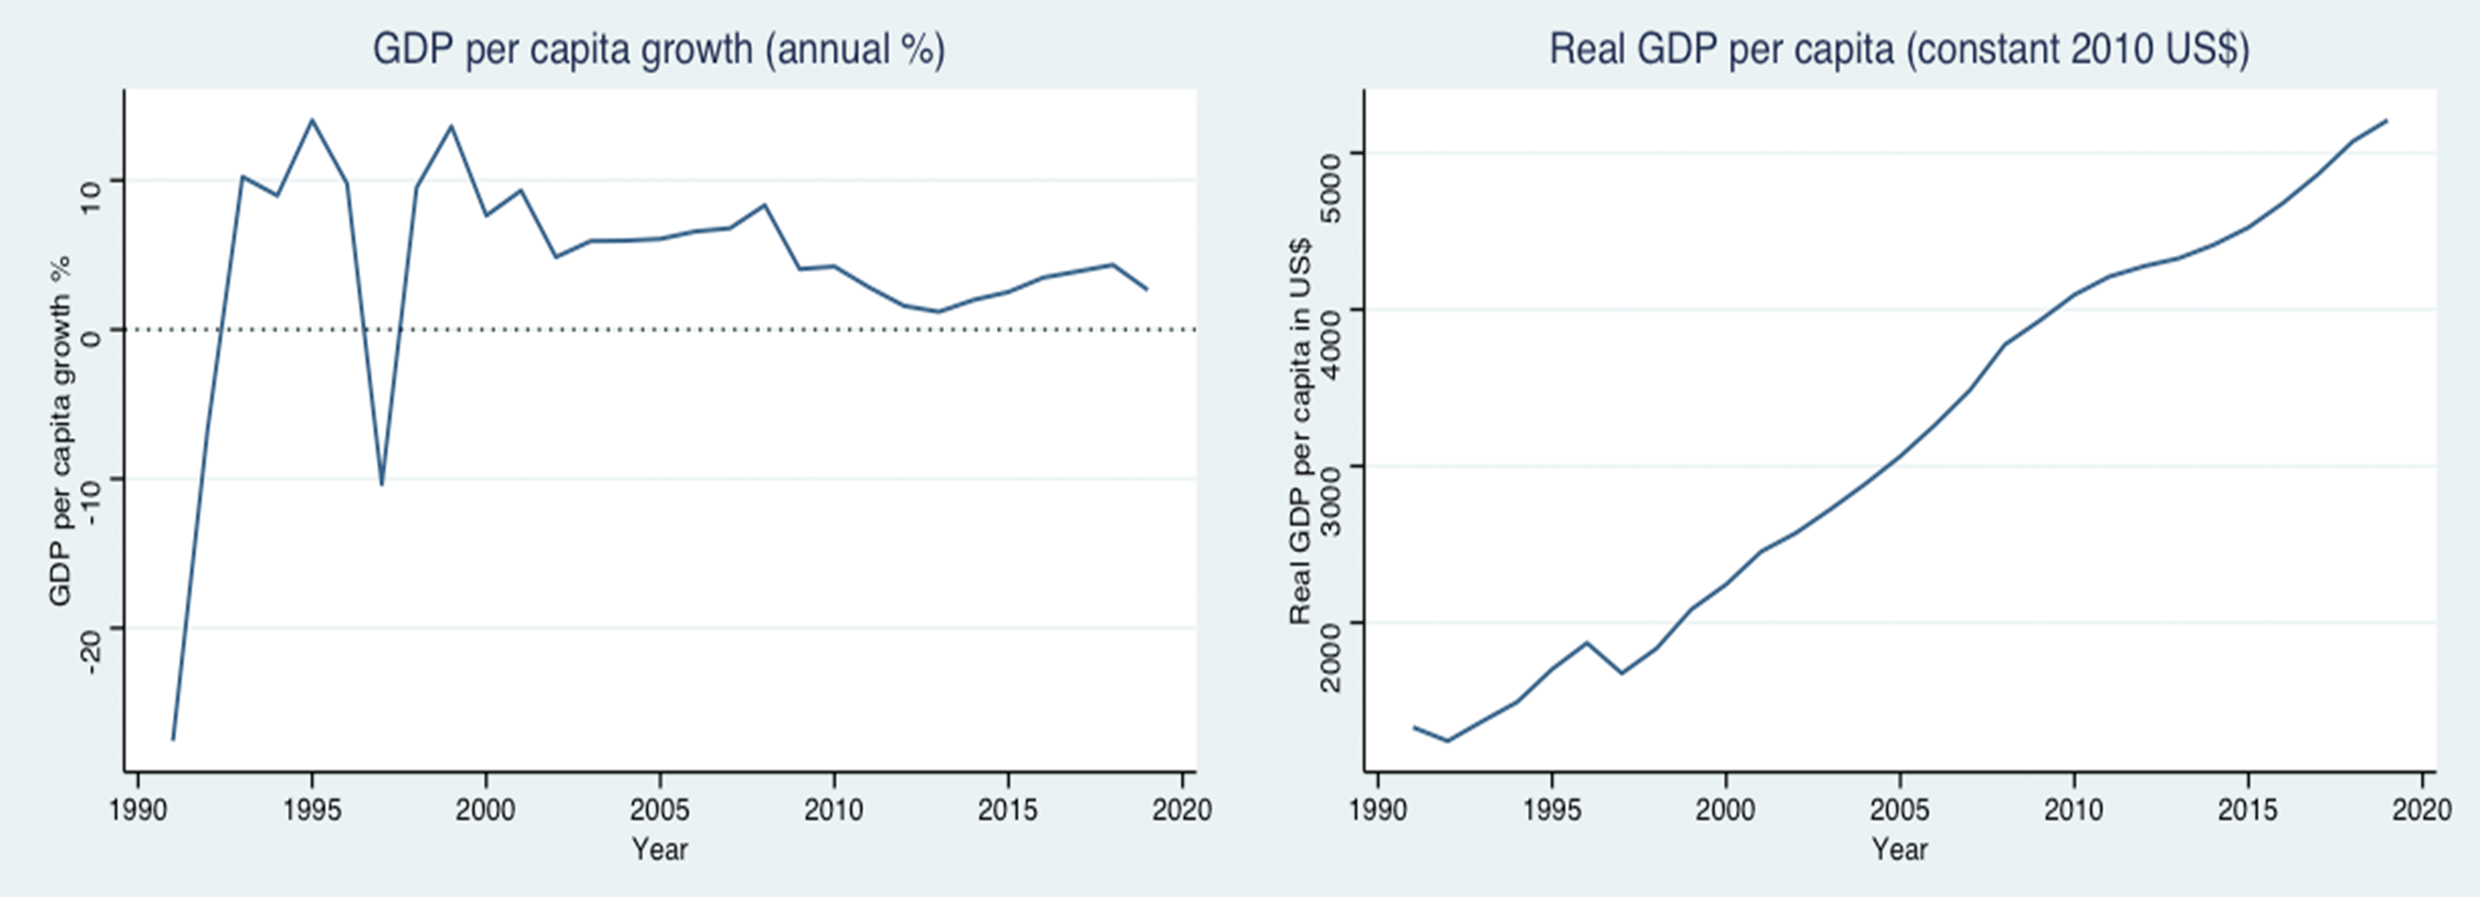
\includegraphics[scale=0.75]{chinchilab-template/Pictures/GDPpercapita.png}
    \caption{GDP per capita growth and Real GDP per capita in Albania.}
    \caption*{\textbf{Source}: World Bank (2020)}
    \label{fig:my_label}
\end{figure}

After getting through the first years, Albania's transition in terms of GDP indicators signalize a robust economic performance. Despite this positive fact, when comparing Albania's GDP (adjusted for purchasing power) with European countries it still is the poorest country on the continent. 
Moreover, recent corruption indicators also convey a gloomy picture. These indicators are extracted from the BEEPS data-set, which is at the core of this thesis, and measures corruption as administrative corruption, or simply bribery. {\bf Figure 2.2} visualizes, for 2013 and 2019, the levels of two corruption indicators in SEE countries. Albania pops up in all of the sub-figures. This picture suggests two insights: First, Albania has in both years the highest level of bribery compared to the other countries. Second, even more alarming, bribery depth surged from 20.4\% in 2013 to 36.1\% in 2019, similarly, bribery incidence surged from 17.6\% in 2013 to 30\% in 2019. For robustness test reasons, {\bf Figure 2.3} depicts the CPI of Albania over the same time span. This figure tells a similar story (note: 100 = best, 0 = worst).\footnote{Unfortunately, due to missing values, it was solely possible to depict region averages of 2019.} One interesting fact can be observed by looking at the range, in which the CPI moves (i.e. between 30 and 40). The first time span until 2016 is characterized by an increasing CPI, whereas the second time span by a decreasing CPI. Furthermore,  \citet[p. 8]{worldbank2000} found the same picture for the year 2000. Across the SEE countries, Albania ranked highest.
\begin{figure}
    \centering
    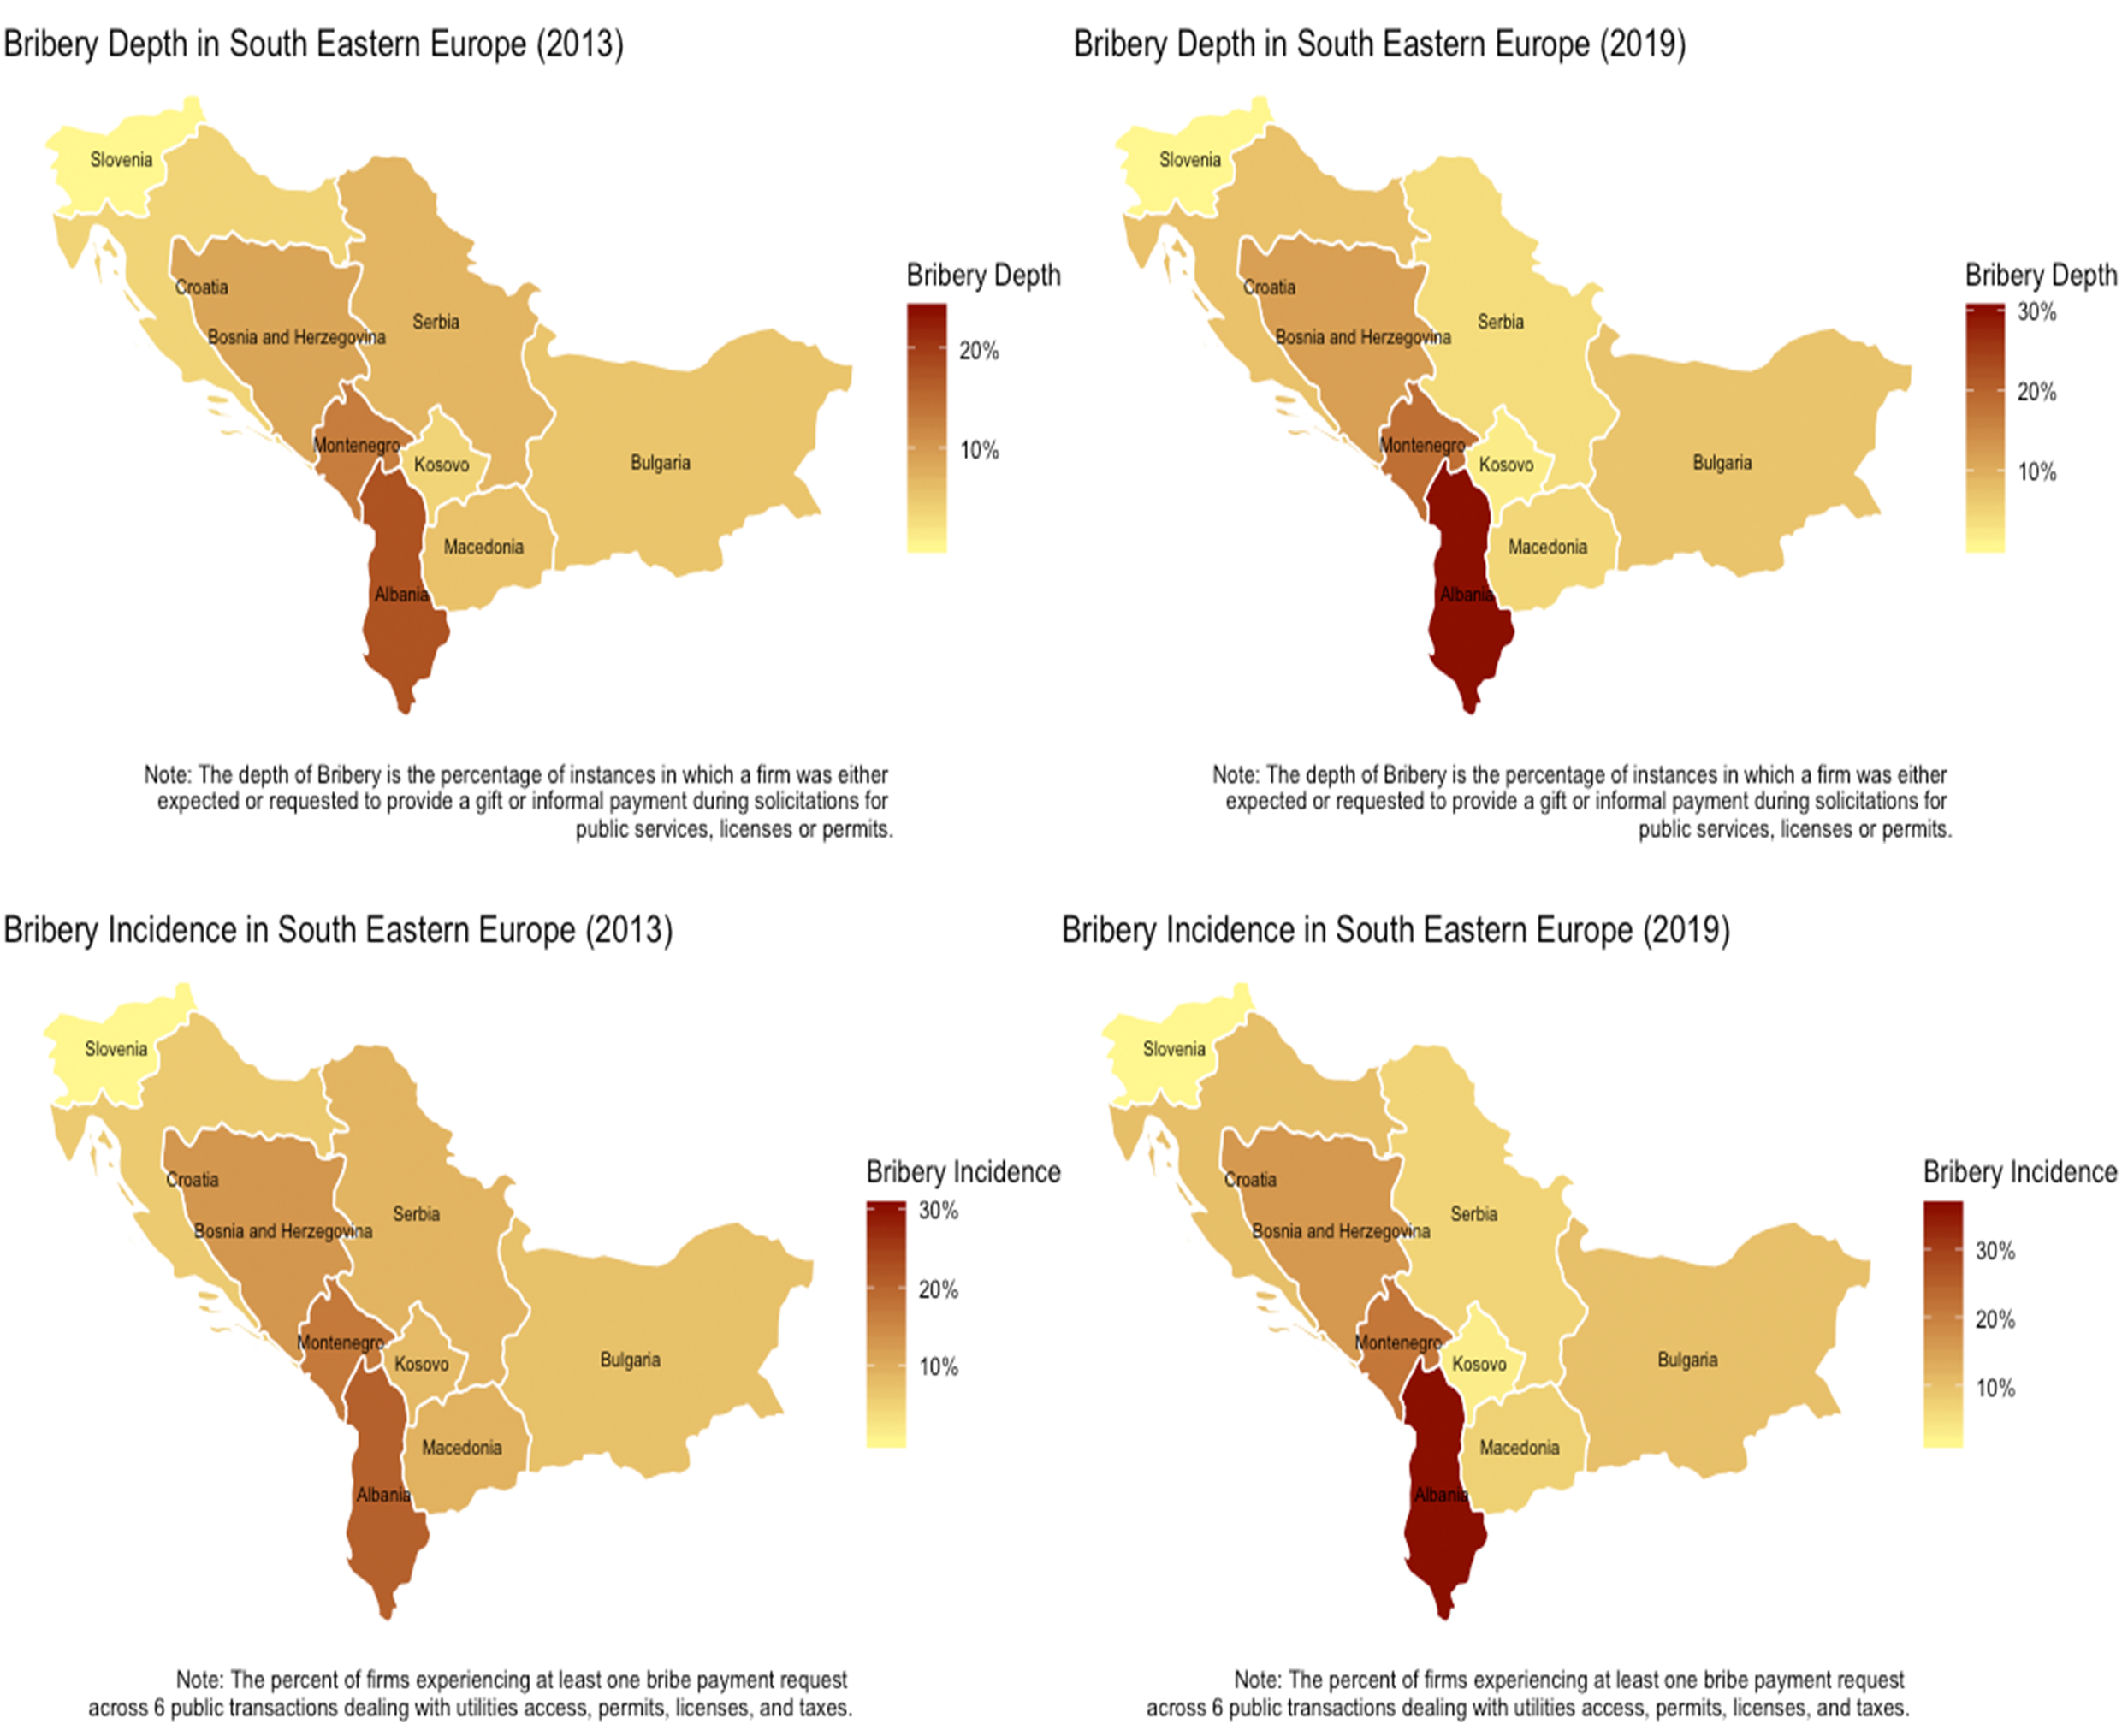
\includegraphics[scale=0.75]{chinchilab-template/Pictures/fullMaps.png}
    \caption{Bribery Depth and Bribery Incidence in SEE from 2013 and 2019.}
    \caption*{\textbf{Source}: Enterprise Surveys, The World Bank.}
    \label{fig:my_label}
\end{figure}
\begin{figure}[h]
    \centering
    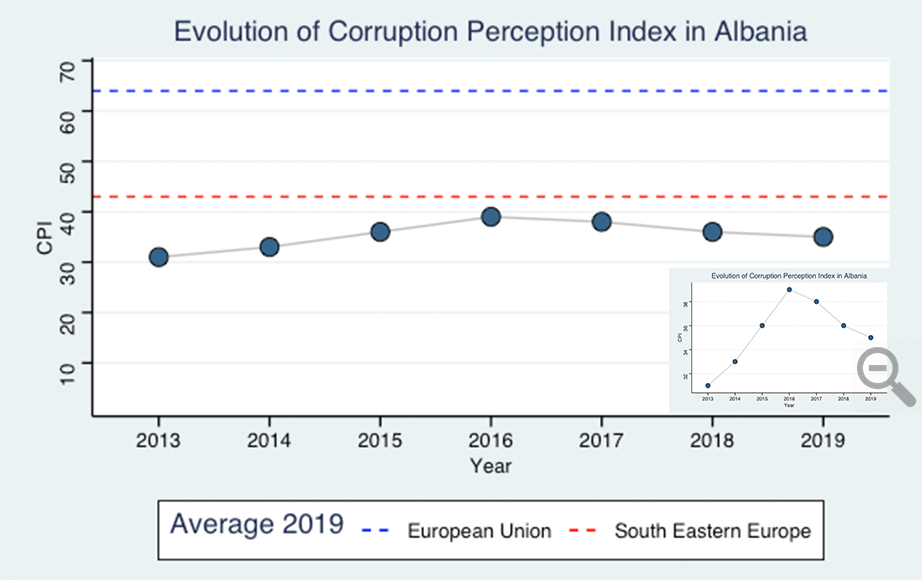
\includegraphics[scale=1.5]{chinchilab-template/Pictures/CPIminus.png}
    \caption{Evolution of CPI in Albania since 2013.}
    \caption*{\textbf{Source}: Corruption Perceptions Index, Transparency International.}
    \label{fig:my_label}
\end{figure}
\begin{figure}[!htb]
    \centering
    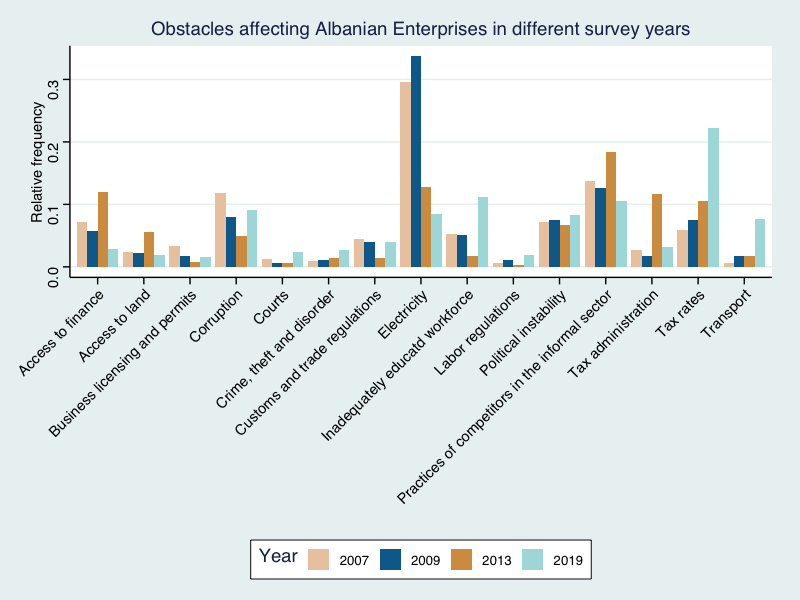
\includegraphics[scale=0.55]{chinchilab-template/Pictures/Obstacle_plot.png}
    \caption{Business obstacles in different years}
    \caption*{\textbf{Source}: Enterprise Surveys (http://www.enterprisesurveys.org), The World Bank.}
    \label{fig:my_label}
\end{figure}

\textbf{Figure 2.4} shows a bar-plot with the relative frequency of various obstacles Albanian firms face in four different survey rounds. In years 2007 and 2009 corruption appears as the third biggest obstacle. In 2013, however, corruption appears at place nine and in 2019 it moved back up to place four - once more showing that corruption grew in recent years. Furthermore, political instability and competition from the informal sector are impediments with constant relative frequency and with at least top 4 positioning since 2007. Moreover, the course of tax rates as an obstacle surged to over 20\% in 2019. By investigating the data\footnote{https://home.kpmg/xx/en/home/services/tax/tax-tools-and-resources/tax-rates-online/corporate-tax-rates-table.html}, we found that the corporate income tax rate increased by 50 basis points from 10\% to 15\% in 2014, which may be a possible explanation for this occurrence. 

To sum up, corruption in Albania seems to have gained new momentum, especially bribing activity in the state-firm relationship. Paradoxically, since the very beginning in 1992, Albania underwent several institutional reforms. Moreover, the first plan of anti-corruption measures to fight corruption was drawn up in 1998 in cooperation with the World Bank. [\citeauthor{mathisen2003donor}, 2003, p. 8] Still, corruption in Albania seems to be steadfast with no long-term improvements. Researchers examining the (in)effectiveness of the first institutional reforms have pointed out that a more individualistic approach is needed. [\citealp{tisne2004ground}] In view of the efforts to become a member of the European Union\footnote{Albania applied in April 2009 for EU membership.}, the European Commission issued an opinion in 2010 with 12 key priorities that Albania had to focus its work on. \citep{european2010communication} The following five measures, which are still in process, have been taken to address the biggest issues related to corruption: justice reform (since 2016), vetting process of judges and prosecutors (2017-2022), fight against corruption and organised crime (Special Anti-Corruption Structure (SPAK)\footnote{An independent judicial institution with the abandonment to investigate corruption.} since 11/2019), public administration reform (2015-2020) and public-financial-management (PFM) reform strategy (2014-2020). \citep{european2019communication}
Despite these reform activities overall corruption as well as administrative corruption seem to have increased. Without evaluating these measures too early, the simultaneous increase in corruption may shed light on its pervasiveness and endemicity in Albania. Hence, it is of our crucial interest to disentangle the effects of administrative corruption on firm's business activity, i.e. measuring the effect of administrative corruption on firm performance. Thereby, we seek to gather insights into the micro-processes of firm-level bribery in order to elaborate policy recommendations. This is especially interesting due to the fact that the EU decided to open accession negotiations with Albania in March 2020.

\textbf{Section 2.4} merges the accumulated insights of this chapter into five research hypotheses.
 
\section{Research Hypotheses}
We expect the relationship between administrative corruption and firm performance to follow the greasing the wheels hypothesis. We argue that reforms so far do not have shown enough effort to diminish the bureaucratic rigidity experienced by the private sector when dealing with state institutions. Therefore, our first hypothesis is as follows:  \\

\textbf{Hypothesis 1:} Administrative corruption will have both, a positive effect on growth and on innovation activity in Albanian enterprises. \\

Next, we contend that complexity of bureaucratic procedures requires firm's to spend more time with government officials. Therefore, raising the costs of firm's, which leads us to the following hypothesis: \\

\textbf{Hypothesis 2a:} Bureaucratic complexity will have a negative effect on growth and innovation activity in Albanian enterprises.\\

Nonetheless, we argue that the greasing effect of corruption on firm performance depends on the level of bureaucratic complexity the firm is embedded in. In an environment of low bureaucratic complexity, bribing deters the performance of firms. Contrary, if firms perceive their environment as suffering from high bureaucratic complexity, bribing greases the dilatory bureaucratic setting and ameliorates firm's performance. Therefore, we hypothesize: \\

\textbf{Hypothesis 2b:} Bureaucratic complexity (higher obstacles) positively moderates the relationship between administrative corruption and firm performance.\\  

Furthermore, informal competition seems to be a serious obstacle for Albanian firm's. We argue that the informal sector may be partially a product of rent-seeking officials. Thus, informal firms hide their activity to cut the additional costs of bureaucratic procedures. Thereby, informal companies achieve competitive cost advantages over formal firms, which may seriously suffer from this type of competition. \\

\textbf{Hypothesis 3a:} The informal sector will have a negative effect on both, growth and innovation activity in Albanian enterprises. \\

Lastly, this negative effect of informal sector firms may be even stronger for formal firms subject to additional bribing costs. Hence, the last hypothesis states: \\

\textbf{Hypothesis 3b:} Informal competition negatively moderates the relationship between administrative corruption and firm performance. \\




